% \chapter{Design Provisions for Self-stressing System for Bridge Application with Emphasis on Precast Panel Deck System}
\chapter{以预制面板系统为重点的桥梁应用自应力系统设计规定}
\label{chp:provisions-self-stressing-system}
% Steel girder bridges often use continuity over the interior supports to reduce interior forces on the spans. In continuous structures with composite concrete decks, the location of maximum negative bending moment is over the interior supports. This moment produces tensile stresses in the concrete deck and compressive stress in the bottom flanges of the girders. The tensile stress in the deck leads to cracking, which allows intrusion of moisture and road salt, causing corrosion of the reinforcement, and supporting girders. Continued maintenance is required to forestall the deterioration; however, replacement of the deck is eventually required.
钢梁桥通常使用内部支撑的连续性来减少跨度上的内力。 在具有组合混凝土桥面板的连续结构中,最大负弯矩的位置在内部支撑上方。 这个力矩在混凝土面板中产生拉应力,在大梁的底部翼缘板中产生压应力。桥面板中的拉应力会导致混凝土开裂,从而使水分和道路盐分侵入,导致钢筋和支撑梁腐蚀。 虽然采取持续维护可以防止结构\gls*{deterioration},但最终还是需要更换桥面板。

% To help alleviate this problem, a self-stressing system was developed as part of the SHRP 2 R19A project. Additional details of the development can be found in the forthcoming final report. The method induces a compressive force in the deck accomplished by raising the interior supports above their final elevation while the deck is cast (cast-in-place construction) or placed (precast construction). Once the concrete has cured, the supports are lowered to their final elevation. Continuity of the steel member and the composite action with the deck produce a compressive stress in the concrete slab, which is balanced by tensile stresses in the bottom of the steel member. As a result, the cracking over interior support is reduced, increasing durability. Additionally, the need for girder splices may be eliminated, making the overall bridge design more efficient and less expensive when compared to conventional design.
为了帮助缓解这个问题,\gls{shrp}2 的 R19A 项目开发了一个自应力系统。有关开发的更多详细信息,请参阅即将发布的最终报告。 该方法通过在浇筑(现场浇筑施工)或安放(预制施工)桥面板时将内部支撑升高到其最终高度以上来在桥面板中产生压缩力。 一旦混凝土固化,支架就会降低到最终高度。钢构件的连续性和与桥面板的复合作用在混凝土板中产生压应力,该压应力由钢构件底部的拉应力平衡。 结果,减少了内部支撑的开裂,增加了耐用性。 此外,与传统设计相比,可以消除对大梁拼接的需要,从而使整体桥梁设计更加高效且成本更低。


% This appendix describes the construction procedure, design considerations, and implementation details for using the self-stressing method. A flow chart is provided to aid in implementation. Simplified formulas applicable to twospan bridges, which represent the most likely use of the method, are also included.
本附录描述了使用自应力法的施工程序、设计注意事项和实施细节。 提供流程图以帮助实施。 还包括适用于双跨桥梁的简化公式,代表最有可能使用该方法。

% \section{CONSTRUCTION PROCEDURE OVERVIEW}
\section{施工方法概述}
% This section provides a brief description of the major steps in the construction procedure, in order to establish a frame of reference and to introduce vocabulary used throughout the appendix. Table A.1 illustrates the major steps required for constructing a bridge using the self-stressing method. These steps will be used as points of reference in the remaining discussion.
本节简要描述构建过程中的主要步骤,以建立参考框架并介绍整个附录中使用的词汇。 \cref{tab:self-stressing-method} 说明了使用自应力法建造桥梁所需的主要步骤。 这些步骤将用作其余讨论的参考点。

\begin{table}
  \caption{Self-Stressing Method Major Steps}\label{tab:self-stressing-method}
  % \input{tables/filename}
\end{table}

The first stage consists of simply placing the girder onto the level supports. The resulting moments and deflections are those obtained from a continuous beam analysis.

During the second stage, the interior support is raised. The bare steel girder responds as a simply supported beam subjected to an upward directed point load at the location of the interior support. Note that the supports could be in the raised position prior to placing the girder. However, due to superposition, the analysis would be the same as described.


Next the concrete deck is cast, or precast panels are placed and grouted. The structure responds like a continuous bare steel beam, just as it would be for conventional construction.

During the fourth stage, the interior support is lowered to its final position. Just as in Stage 2, the response is that of a beam supported at the exterior supports only and subjected to a point load. However, the structure is now composite and the point load is directed downward. This action places the concrete deck over the supports into compression.

Over time, creep and shrinkage occur in the concrete deck. This may be accounted for in two stages. First, the creep and shrinkage are seen as an applied curvature on the structure. If the beam were simply supported by the exterior supports, this applied curvature would result in additional deflection without inducing additional load. However, due to the continuity, a restoring force is generated that prevents the displacement and results in additional stresses.

% \section{DESIGN CONSIDERATIONS}
\section{设计注意事项}
This section provides a discussion of the design issues specific to the use of the self-stressing method. Design of bridges using the self-stressing method should follow the provisions for I-Section and Box-Section flexural members contained in Section 6.10 and 6.11 respectively, of the AASHTO LRFD Bridge Design Specifications (LRFD Specifications), except as modified herein \cite{aashto2012l}.

\subsection{General}
The use of the self-stressing method is limited to straight I- and Box-Section steel girders and is applicable only to continuous multi-span structures with a composite deck. Practical limitations dictate that the method is most likely to be used in two-span structures. Simplified design aids are provided in Section A.5 for structures with two spans.

\subsection{Analysis}
Two options provided for the analysis of the structure are described in the following section. Note that the analysis methods should only be used when analyzing the construction steps associated with the self-stressing method and not the overall analysis procedures as covered in Chapter 4 of the LRFD Specifications.

\subsubsection{Simplified}
The simplified analysis method relies on first order techniques that disregard time effects in the concrete. These effects are accounted for using conservative correction factors presented in the implementation details portion of the provisions (Section A.3). The correction factors account for the effects of creep and shrinkage in the evaluation of stresses and deflections. As an alternative, advanced methods of analysis may be used that directly evaluate these effects.


\subsubsection{Advanced}

Advanced methods explicitly consider the effects of creep and shrinkage to evaluate the stresses and deflections.

Several examples are the effective modulus method (EMM), adjusted effective modulus method (AEMM), stepby-step method (SSM), and the rate of creep method (RCM).

When the creep and shrinkage strains are known, or otherwise assumed, then the LRFD Specifications, Section C4.6.6 can be used for calculating the resulting stresses and deformations.

\subsection{Forces}

The forces and stresses in all components that arise due to the self-stressing construction procedure should be considered in evaluating the load effects during design. For the purpose of design, the locked-in prestressing force shall be considered a dead load force applied to the composite long-term section (DC2).


The LRFD Specifications, Section 3.4.1 states that where prestressed components are used in conjunction with steel girders, the force effect should be considered as locked-in construction loads (EL). However, in this situation the prestressing forces are being developed by gravity effects rather than applied by prestressing devices. As such, the variability in the resulting stresses will be of the same magnitude as the variability of the dead load effects, which leads to the decision of considering the prestress stress as DC2 loading.


Note that the self-stressing procedure will generate tensile stresses in the bottom of the steel girders that will serve to offset some of the compressive dead and live load stresses. As such, the stresses due to the self-stressing procedure should be kept separate from other dead load stress sources and the minimum load factor for dead load should be used (0.9).

\subsection{Deflections}

The final deflected shape is necessary for determining the camber requirements of the girders and can be obtained by summing the deflections from the various construction stages.

\section{DESIGN PROCEDURE AND IMPLEMENTATION DETAILS}

This section provides a step-by-step procedure for designing a bridge incorporating the self-stressing method. All grout, and/or adhesives must be adequately cured prior to lowering the interior support. The creep and shrinkage properties of the materials must be compatible with the intended use and properties assumed during analysis.

\paragraph*{Step1. Determine Required Amount of Prestress}
The self-stressing method is a way to introduce compressive stresses in the concrete deck of a multi-span continuous beam. The compressive stresses are generally located near the interior supports and therefore work to counter the tensile stresses that arise in this vicinity due to gravity and live loading. The result is a reduction in cracking and an accompanying increase in service life. The magnitude of the prestress that must be applied in order to achieve the desired effects has been determined based on past experience with decks that have been prestressed using traditional mechanical methods.

\subparagraph*{Minimum Final Prestress}
% The recommended minimum level of prestress at the top fiber of the concrete deck over an interior support, after all losses, is 750 psi.
在计入所有损失之后,带有内部支撑的混凝土桥面板板顶推荐最低预应力水平为 \qty{5.2}{MPa}。

% The simplified (Bernoulli assumption) analysis methods predict a linear variation of stresses through the thickness of the deck, which produces a maximum stress value at the face of the concrete. In practice, creep effects quickly blunt this maximum stress value, resulting in a more uniform stress profile through the depth of the concrete. The prescribed minimum prestress value at the face of the slab is intended to provide a final uniform value over the top half of the slab of 250 psi, which is the value recommended in Section 9.7.5.3 of the LRFD Specifications for longitudinal prestressing of concrete slabs.
采用伯努利假设的简化分析方法预测应力随桥面厚度为线性变化,在混凝土表面产生最大应力值。实际上,徐变效应会迅速减小该最大应力值,从而在混凝土高度上产生更均匀的应力分布。板面处规定的最小预应力值旨在为板的上半部分提供 \qty{1.72}{MPa} 的最终均匀值,这是 \lrfd 第 9.7.5.3 节中用于混凝土板的纵向预应力的推荐值。

% \cref{fig:stress-distribution-concrete-deck} shows the initial stress distribution in the concrete deck and the distribution that develops after some period of time has elapsed.
\cref{fig:stress-distribution-concrete-deck}显示了混凝土桥面中的初始应力分布以及经过一段时间后形成的分布。

\begin{figure}
  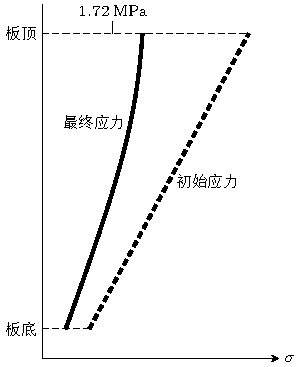
\includegraphics{stress-distribution-concrete-deck.pdf}
  % \caption{Stress distribution in concrete deck}
  \caption{桥面板内的应力分布}
  \label{fig:stress-distribution-concrete-deck}
\end{figure}

\subparagraph*{Maximum Initial Prestress}

The maximum initial prestress to be applied shall be no greater than 60 percent of the concrete compressive strength.

There is no upper limit recommendation in the literature because the material maximum strength is a natural upper bound. However, in order to maintain a safe margin, the upper limit shall not be greater than 60\% of the concrete compressive strength ($0.6f'_\text{c}$), which is the compressive stress limit recommended in Section 5.9.4.1.1 of the LRFD Specifications for pretensioned and posttensioned concrete components, including segmentally constructed bridges.

\subparagraph*{Adjust Prestress for Losses}

In lieu of an exact analysis, the prestress loss may be conservatively estimated as 20\% when the initial prestress value is less than 40\% of the concrete compressive strength, and 30 percent when the initial prestress value is greater than 40\% of the concrete compressive strength.

\cref{eq:initial-prestress} gives the initial prestress at the top fiber that is to be applied.
\begin{equation}
  \label{eq:initial-prestress}
  \sigma_\text{pi}= \frac{\sigma_\text{pf}}{1-r_\text{s}}
\end{equation}
\begin{EqDesc}{\sigma_\text{pf}}
  \item[\sigma_\text{pf}] final prestress stress
  \item[\sigma_\text{pi}] initial prestress stress
  \item[r_\text{s}] loss due to creep and shrinkage
\end{EqDesc}

\paragraph*{Step2. Calculate Amount of Deflection to Obtain Desired Prestress}
Determine the height to which the interior support must be raised so that upon release it will provide the desired amount of prestress.

The problem at hand is essentially that of support settlement. How far must the interior support settle so that the stress in the top of the deck is the value chosen in the previous design step?

For the following steps, the structure to be considered is the composite structure being supported at the exterior supports only, which is shown in \cref{fig:equivalent-structure1}.

\begin{figure}
  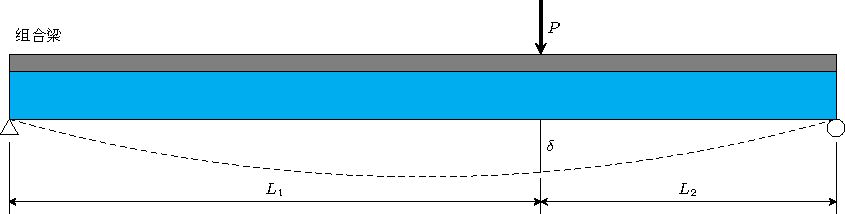
\includegraphics{equivalent-structure1.pdf}
  % \caption{Equivalent structure used for calculating stresses during lowering of support.}
  \caption{Equivalent structure used for calculating stresses during lowering of support.}
  \label{fig:equivalent-structure1}
\end{figure}

\begin{enumerate}[a)]
  \item Determine the stress at the top fiber of the deck due to point loading applied at the interior support location.
  \item Use the result from (a) to solve for the magnitude of the forces required to produce the desired prestress determined in Step 1.
  \item Calculate the stiffness with respect to point load applied at the interior support location.
  \item Use the stiffness from (c) to solve for displacement required to produce the necessary force. For the
  structure shown in \cref{fig:equivalent-structure1}, this displacement is given in \cref{eq:displacement-required}.
  \begin{equation}
    \label{eq:displacement-required}
    \delta = \frac{\sigma_\text{ts}L_1L_2}{3 E_\text{conc}c_\text{cs}}
  \end{equation}
  \begin{EqDesc}{E_\text{conc}}
    \item[\delta] amount of displacement required
    \item[\sigma_\text{ts}] initial prestress stress
    \item[L_1] length of span 1 
    \item[L_2] length of span 2
    \item[E_\text{con}] modulus of elasticity of concrete
    \item[c_\text{ts}] distance from neutral axis to top fiber of slab
  \end{EqDesc}
\end{enumerate}

\paragraph*{Step3. Determine Forces Due to Lifting Bare Steel Beam}
The results obtained from this step are used to complete the constructability check of the structure. For the following steps, the structure to be considered is the bare steel beam being supported at the exterior supports only, as shown in \cref{fig:equivalent-structure2}.

\begin{figure}
  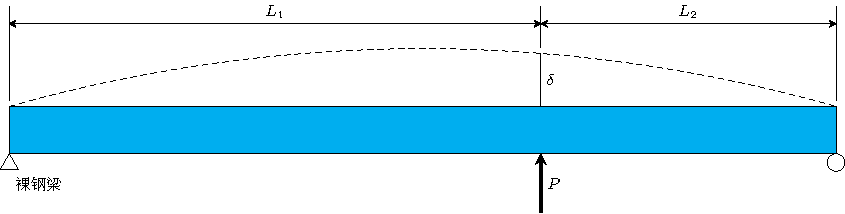
\includegraphics{equivalent-structure2.pdf}
  \caption{Equivalent structure used for calculating stresses during the raising of support.}
  \label{fig:equivalent-structure2}
\end{figure}

\begin{enumerate}[a)]
  \item\label{lst:calc-stiffness} Calculate the stiffness with respect to point loads applied at the interior support locations.
  \item\label{lst:calc-force-required} Use the stiffness from \ref{lst:calc-stiffness} to calculate the force required to lift the interior supports to the height determined in the previous design step. For the structure shown in \cref{fig:equivalent-structure2}, this force is given in \cref{eq:force-required}.
  \begin{equation}
    \label{eq:force-required}
    P = \frac{3E_\text{steel} I_\text{steel} (L_1+L_2)} {L_1^2L_2^2} \delta
  \end{equation}
  \begin{EqDesc}{E_\text{steel}}
    \item[P] reaction at support due to deflection of support
    \item[\delta] deflection of support
    \item[L_1] length of span 1
    \item[L_2] length of span 2
    \item[E_\text{steel}] modulus of elasticity of steel
    \item[I_\text{steel}] moment of inertia of bare steel girder
  \end{EqDesc}
  \item Using the force given by \ref{lst:calc-force-required}, the reactions, moments, and stresses can be calculated as needed for
  design.
\end{enumerate}

The steel girders, and any support structures, temporary or permanent, must be designed for the concentrated
forces that are developed due to lifting the girders.

\subparagraph*{End Anchorages}
The calculated vertical displacement may require a lifting force that is greater than the self-weight of the steel
girder such that the girder would lift off of the end supports. In this situation, the exterior ends of the girder may be
anchored to prevent uplift. Once the concrete deck is in place, the weight of the deck will replace this anchorage
force.

Also note that loading within the spans can affect uplift at the end supports. Consider the structure shown in
\cref{fig:loading-span-1}. Loading in the first span will create uplift at the end support of the opposite span. Therefore, the
progression of deck casting or precast panel placement may affect the need for end anchorages. This possibility must
be properly accounted for through either design or the specification of explicit procedures to avoid the condition
described.

\begin{figure}
  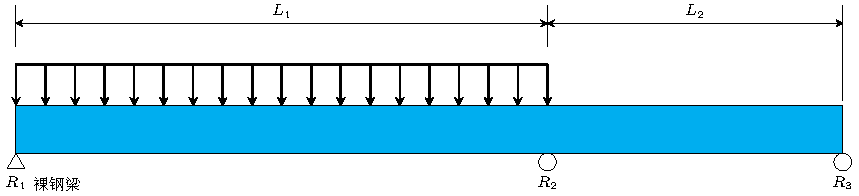
\includegraphics{loading-span-1.pdf}
  \caption{Loading in Span 1 Producing Uplift at Support R3.}
  \label{fig:loading-span-1}
\end{figure}

\cref{eq:reaction-end-span2} gives the reaction at the end of Span 2 (unloaded span) due the following combination of loading:
\begin{itemize}
  \item Self-weight of the steel girder ($w_\text{steel}$)
  \item An upward displacement of the interior support ($\delta$)
  \item Uniform load with Span 1 due to deck placement ($w_\text{deck}$)
\end{itemize}

This equation will aid in evaluating the need and magnitude of end anchorages. The critical condition occurs
when Span 1, the loaded span, is longer than Span 2. Therefore, when the spans are different lengths, the deck within
the shorter span should be cast first.

\begin{equation}
  \label{eq:reaction-end-span2}
  \frac{w_\text{steel}(3L_2^2+L_1L_2-l_1^2)}{8L_2}-\frac{3E_\text{steel}I_\text{steel}}{L_1L_2^2}\delta-\frac{w_\text{deck}L_1^3}{8L_2(L_1+L_2)}
\end{equation}
\begin{EqDesc}{E_\text{steel}}
  \item[w_\text{steel}] uniform load due to self-weight of the steel
  \item[w_\text{deck}] uniform load due to deck placement
  \item[\delta] deflection of support (positive upward)
  \item[L_1] length of span 1
  \item[L_2] length of span 2
  \item[E_\text{steel}] modulus of elasticity of steel
  \item[I_\text{steel}] moment of inertia of bare steel girder
\end{EqDesc}

For the case of two equal spans ($L_1=L_2=L$), \cref{eq:reaction-end-span2} can be simplified to
\begin{equation}
  \frac{3Lw_\text{stell}}{8}-\frac{3E_\text{stell}I_\text{steel}}{L^3}\delta-\frac{Lw_{deck}}{16}
\end{equation}
\begin{EqDesc}{L}
  \item[L]  length of spans 1 and 2 (equal)
\end{EqDesc}

End Anchorages, when necessary must be designed to withstand the concentrated force that is to be applied.

\paragraph*{Step4. Determine Forces and Stresses Due to Lowering Composite Bridge}

The forces and stresses imparted on the structure due to lowering the composite bridge are obtained from a similar analysis to that performed when the amount of deflection was originally calculated in Step 3.

For the following steps, the structure to be considered is the composite structure being supported at the exterior supports only, as shown in \cref{fig:equivalent-structure3}.

\begin{figure}
  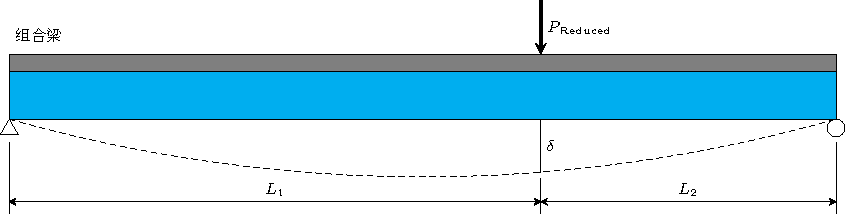
\includegraphics{equivalent-structure3.pdf}
  \caption{Equivalent structure used for calculating stresses during lowering of support.}
  \label{fig:equivalent-structure3}
\end{figure}

\begin{enumerate}[a)]
  \item Calculate the stiffness with respect to a point load applied at the interior support location.
  \item Use the stiffness from (a) to calculate the equivalent point force due to the lowering of the support.
  \item Reduce the force calculated in (b) to account for the prestress loss due to creep and shrinkage, as
  determined in Step 2.
  \item Using the reduced force applied to the composite structure supported at the exterior supports, calculate
  the internal forces and stresses necessary for design.
\end{enumerate}

The resulting forces and stresses from this step should be considered dead load forces applied to the composite
structure for the purpose of design.

\paragraph*{Step5. Determine Deflected Shape}
The final deflected shape is necessary for determining the camber requirements of the girders. The final deflection is the summation of deflections from the various construction stages.

\subparagraph*{Bare Steel Deflection}
Sources of deflection of the bare steel girder are:
\begin{itemize}
  \item Self-weight of steel,
  \item Initial lift of interior supports, and
  \item Casting of wet concrete.
\end{itemize}

The deflection due to the self-weight of the steel and casting of the wet concrete is calculated in a conventional manner using the continuous bare steel structure, as shown in \cref{fig:deflection-bare-steel}. Equations for calculating the deformation along the length of the beam can be found the \cref{sec:design-aids}.

\begin{figure}
  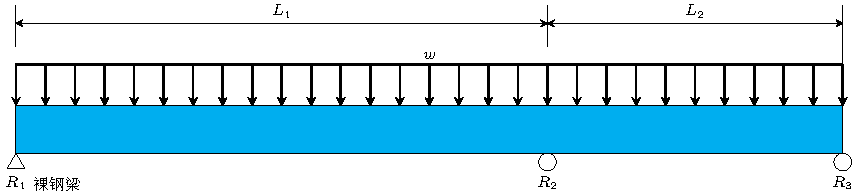
\includegraphics{deflection-bare-steel.pdf}
  \caption{Structure for calculation of bare steel deflections.}
  \label{fig:deflection-bare-steel}
\end{figure}

Calculation of the deflection due to the initial lift of the interior support is determined considering the bare steel
girder supported at the exterior supports only, as shown in \cref{fig:composite-deflections-lowering-support}. The structure is subjected to point forces
applied at the interior supports as determined in Step 3. Equations for calculating the deformation along the length
of the beam can be found in \cref{sec:design-aids}.

\begin{figure}
  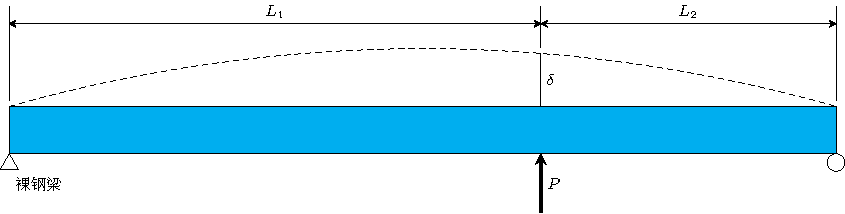
\includegraphics{equivalent-structure2.pdf}
  \caption{Structure for calculation of composite deflections due to lowering the support.}
  \label{fig:composite-deflections-lowering-support}
\end{figure}

\subparagraph*{Composite Deflection}
Calculation of the deflection due to the lowering of the interior support is determined by considering the composite bridge girder supported at the exterior supports only, as shown in \cref{fig:composite-girder-exterior-supports-only}. The structure is subjected to point forces applied at the interior supports as determined in Step 3 without the reduction in load meant to account for creep and shrinkage. Creep and shrinkage have the opposite effect, resulting in an increase of the total deflection. This effect is discussed in the following section. Equations for calculating the deformation along the length of the beam can be found in Step 2.

\begin{figure}
  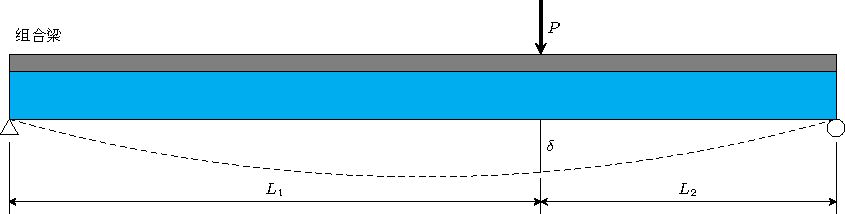
\includegraphics{equivalent-structure1.pdf}
  \caption{Structure for calculation of bare steel deflections due to initial lifting of support.}
  \label{fig:composite-girder-exterior-supports-only}
\end{figure}

\subparagraph*{Relaxation Deflection}
Additional deflections arise due to curvature induced along the beam due to the effects of creep and shrinkage. The resulting loading can be seen in \cref{fig:curvature-applied-continuous-structure}.

\begin{figure}
  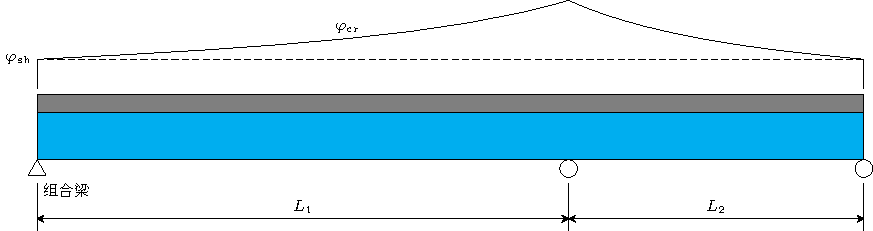
\includegraphics{curvature-applied-continuous-structure.pdf}
  \caption{Curvature applied to continuous structure due to creep and shrinkage.}
  \label{fig:curvature-applied-continuous-structure}
\end{figure}

The steps for calculating the deflected shape can be performed using the following steps, considering the
structure supported at the exterior supports only, as shown in \cref{fig:structure-determination-restoring-force}.

\begin{figure}
  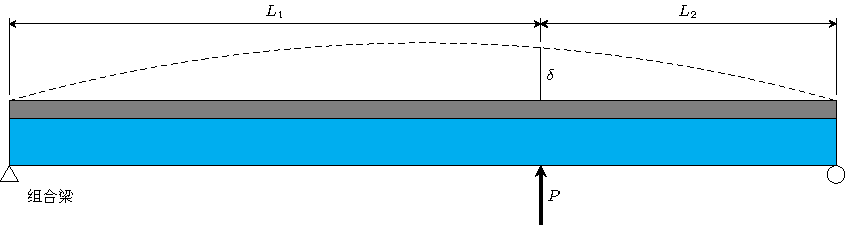
\includegraphics{structure-determination-restoring-force.pdf}
  \caption{Structure for determination of restoring force}
  \label{fig:structure-determination-restoring-force}
\end{figure}

\begin{enumerate}[a)]
  \item\label{lst:calc-stiffness-point-load} Calculate the stiffness with respect to a point load applied at the interior support location.
  \item Determine the curvature along the length of the beam. The curvature at a section can be obtained from \cref{eq:section-curvature}. LRFD Specifications, Section 5.4.2.3.1 provides methods for determining the values of $\varepsilon_\text{sh}$ and $\varepsilon_\text{cr}$ .
  \begin{equation}
    \label{eq:section-curvature}
    \varphi =\frac{1}{I_\text{c}} \int (\varepsilon_\text{sh}+ \varepsilon_\text{cr}) z \dif z
  \end{equation}
  \begin{EqDesc}{\varepsilon_\text{sh}}
    \item[\varphi] curvature of section
    \item[I_\text{c}] composite moment of inertia
    \item[\varepsilon_\text{sh}] strain due to shrinkage
    \item[\varepsilon_\text{cr}] strain due to creep
    \item[z] distance from neutral axis
  \end{EqDesc}
  \item\label{lst:calc-displaced-shape} Calculate the displaced shape of the structure due to the applied curvature, shown in \cref{fig:deflection-curvature}. The displacement can be calculated using the integration given in \cref{eq:displacement-applied-curvature}.
  \begin{figure}
    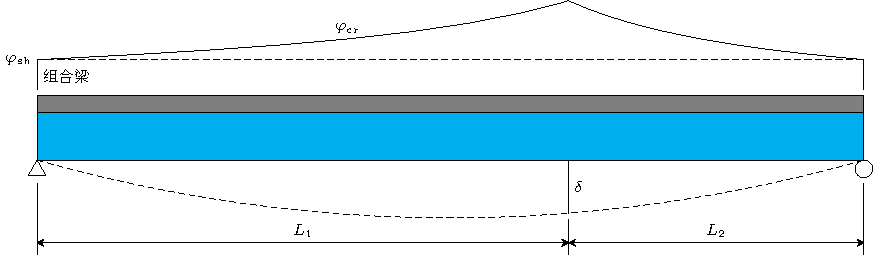
\includegraphics{deflection-curvature.pdf}
    \caption{Structure for determination of deflection due to curvature}
    \label{fig:deflection-curvature}
  \end{figure}
  \begin{equation}
    \label{eq:displacement-applied-curvature}
    \delta(x) = \int_0^x\int_0^x \varphi(x) \dif x\dif x
  \end{equation}
  \begin{EqDesc}{\varphi(x)}
    \item[\varphi(x)] curvature along the length of the beam
  \end{EqDesc}
  \item\label{lst:determine-force} Using the stiffness from \ref{lst:calc-stiffness-point-load}, determine the force required to offset the displacement at the support location calculated in \ref{lst:calc-displaced-shape}.
  \item The resulting deflection due to the relaxation is the sum of the deflections obtained from the applied curvature (\cref{eq:section-curvature}) and the application of the point load determined in \ref{lst:determine-force} upon the structure
  shown in \cref{fig:structure-determination-restoring-force}.
\end{enumerate}

\paragraph*{Step6. Carry Out Remainder of Design}

The remainder of the design proceeds as it would for a conventional steel girder bridge with concrete deck.


% \section{DESIGN FLOWCHART}
\section{设计流程图}
整个设计过程的流程图如\cref{fig:design-flowchart} 所示:

\begin{figure}
  % \includegraphics[width=\linewidth]{graphic-file}
  % \caption{Design flowchart}
  \caption{设计流程图}
  \label{fig:design-flowchart}
\end{figure}

% \section{DESIGN AIDS FOR TWO-SPAN BRIDGES}
\section{两跨桥梁的设计辅助工具}
\label{sec:design-aids}
两跨桥梁的设计辅助图表如\cref{fig:uniform-load-onespan-equal-spans,fig:uniform-load-twospan-equal-spans,fig:uniform-load-onespan-unequal-spans,fig:uniform-load-twospan-unequal-spans}所示:

\begin{figure}
  % \includegraphics[width=\linewidth]{graphic-file}
  % \caption{Continuous beam—two equal spans—uniform load on one span}
  \caption{两等跨连续梁——一跨均布荷载}
  \label{fig:uniform-load-onespan-equal-spans}
  % \caption{Continuous beam—two equal spans—uniformly distributed load}
  \caption{两等跨连续梁——均布荷载}
  \label{fig:uniform-load-twospan-equal-spans}
  % \caption{Continuous beam—two equal spans—uniform load on one span}
  \caption{不等跨两跨连续梁——一跨均布荷载}
  \label{fig:uniform-load-onespan-unequal-spans}
  % \caption{Continuous beam—two equal spans—uniformly distributed load}
  \caption{不等跨两跨连续梁——均布荷载}
  \label{fig:uniform-load-twospan-unequal-spans}
\end{figure}